% Подключение файла с настройками и подключенными пакетами
\documentclass[
candidate, % document type
subf, % use and configure subfig package for nested figure numbering
times % use Times font as main
]{disser}

% Кодировка и язык
\usepackage[T2A]{fontenc} % поддержка кириллицы
\usepackage[utf8]{inputenc} % кодировка исходного текста
\usepackage[english,russian]{babel} % переключение языков

% Геометрия страницы и графика
\usepackage[left=3cm, right=1cm, top=2cm, bottom=2cm]{geometry} % поля страницы
\usepackage{graphicx} % подключение графики
\usepackage{pdfpages} % вставка pdf-страниц
\usepackage{tikz}
\usetikzlibrary{arrows.meta, positioning, fit}
\usepackage{float} % поддержка [H] для figure и table

% Таблицы
\usepackage{array} % расширенные возможности для работы с таблицами
\usepackage{tabularx} % автоматический подбор ширины столбцов
\usepackage{dcolumn} % выравнивание чисел по разделителю
\usepackage{longtable}

% Математика
\usepackage{bm} % полужирное начертание для математических символов
\usepackage{amsmath} % дополнительные математические возможности
\usepackage{amssymb} % дополнительные математические символы

% Библиография и ссылки
\usepackage{cite} % поддержка цитирования
\usepackage{xurl}
\usepackage[unicode,hidelinks]{hyperref} % создание гиперссылок без видимых рамок

% Прочее
\usepackage{color} % работа с цветом
\usepackage{epstopdf} % конвертация eps в pdf
\usepackage{multirow} % объединение ячеек таблиц по вертикали
\usepackage{afterpage} % вставка материала после текущей страницы
\usepackage[font={normal}]{caption} % настройка подписей к рисункам и таблицам
\usepackage[onehalfspacing]{setspace} % полуторный интервал
\usepackage{fancyhdr} % установка колонтитулов
\usepackage{listings} % поддержка вставки исходного кода
\usepackage{pdflscape}
\usepackage{enumitem}

% Установка шрифта Times New Roman
\renewcommand{\rmdefault}{ftm}

% Приведение основного текста к 14 pt при полуторном интервале
\makeatletter
\renewcommand\normalsize{%
  \@setfontsize\normalsize{14pt}{21pt}%
  \abovedisplayskip 12pt plus 3pt minus 7pt%
  \abovedisplayshortskip \z@ plus 3pt%
  \belowdisplayshortskip 7pt plus 3pt minus 4pt%
  \belowdisplayskip \abovedisplayskip
  \let\@listi\@listI
}
\normalsize
\typeout{BASE FONT SIZE = \f@size pt}
\makeatother
\setlength{\emergencystretch}{3em}

% Создание нового типа столбца для выравнивания содержимого по центру
\newcommand{\PreserveBackslash}[1]{\let\temp=\\#1\let\\=\temp}
\newcolumntype{C}[1]{>{\PreserveBackslash\centering}p{#1}}
% Читаемые текстовые колонки для таблиц (без выравнивания по ширине)
\newcolumntype{P}[1]{>{\raggedright\arraybackslash}p{#1}} % фиксированная ширина, переносы, левое выравнивание
\newcolumntype{Y}{>{\raggedright\arraybackslash}X}        % "резиновая" ширина как X, но тоже левое выравнивание

% Настройка стиля страницы
\pagestyle{fancy}      % Использование стиля "fancy" для оформления страниц
\fancyhf{}              % Очистка текущих значений колонтитулов
\fancyfoot[C]{\thepage} % Установка номера страницы в нижнем колонтитуле по центру
\renewcommand{\headrulewidth}{0pt} % Удаление разделительной линии в верхнем колонтитуле

% Настройка подписей к изображениям и таблицам
\captionsetup{format=hang,labelsep=period}
\captionsetup[table]{
  justification=raggedright,
  singlelinecheck=false
}

% Использование полужирного начертания для векторов
\let\vec=\mathbf

% Установка глубины оглавления
\setcounter{tocdepth}{2}

% Указание папки для поиска изображений
\graphicspath{{images/}}

% Установка стилей страницы и главы
\pagestyle{footcenter}
\chapterpagestyle{footcenter}

% ??????? ?????? ?????? ????? ????????, ??????? ?????? ????? disser
\\setlength{\\parskip}{0pt}


\begin{document}

% Задаёт порядок библиографического списка по группам из методички:
% нормативные акты, периодические издания, электронные ресурсы, иностранные источники.
\nocite{constitutionRu,federalLaw152FZ_2006,federalLaw259FZ_2020,notariatLawArticle31}
\nocite{Orlov2024Moluch,Haritonova2024HSE}
\nocite{fnpOfficialAbout,HSEInternetInfrastructurePandemic2021,HSETelecomInfrastructure2022,TAdviserInternetTrafficRussia2026,cniNotariat2024Stats,rosimushchestvo2025Escheat,bankRussia2024HouseholdFunds,moex2024RetailInvestors,bankRussia2024CFAReview,bankRussia2025CFAReview,bankRussia2025CryptoFlows,akitEcommerceRussia2025,habrCareerSalariesH2_2025,fnsInsuranceRates2026,pravoRu2024EscheatMoscow}
\nocite{Edwards2013PostMortemPrivacy,Harbinja2022DigitalDeath,gdprReg2016_679,FrenchDigitalInheritanceLaw2016,bghIIIzr18317_2018,RUFADAA2015,googleInactiveAccountManager,facebookLegacyContact,appleLegacyContact,nist80063_4_2025,iso27001_2022,nist80053r5_2020,enisaThreatLandscape2023,iso14721_2025,iso16363_2025,iso19005_4_2020,nist80030r1_2012,owaspASVS403}

% Включение титульного листа (первая страница файла Title.pdf)

\includepdf[pages={1-1}]{extra/Title.pdf}

% Аннотация, Содержание, Введение
% \newpage
% \begin{center}
%   \textbf{\large АННОТАЦИЯ}
% \end{center}


% Объектом исследования данной работы стали системы частиц, взаимодействующих посредством обобщенного потенциала Леннарда-Джонса с переменной степенью притяжения.
% С помощью данных систем выявлялось влияние дальнодействия притяжения на фазовые диаграммы, роль дальнодействия в транспортных свойствах, а также влияние на спектры возбуждений.
% Для решения поставленной задачи методом молекулярной динамики были смоделированы системы.
% Пост обработка проводилась с использованием MATLAB и python.

% В ходе работы были проведены моделирования систем с различным дальнодействием притягивающей ветви потенциала взаимодействия.
% Рассчитаны фазовые диаграммы систем, их транспортные свойства и спектры возбуждений на бинодали жидкость-газ.
% Предложен новый метод классификации частиц на конденсат, газ и поверхность в системах с фазовым расслоением.
% На основании полученных результатов, было впервые выявлено влияние дальнодействия притяжения в молекулярных системах на фазовые диаграммы, положения тройных и критических точек и корреляции транспортных свойств со спектрами возбуждений на бинодали жидкость-газ.
% С помощью нового метода классификации частиц, основанного на методе кластеризации DBSCAN (Density-Based Spatial Clustering of Applications with Noise), был разработан метод построения фазовых диаграмм и анализа нуклеации.

% \onehalfspacing
% \setcounter{page}{2}

\newpage
\onehalfspacing
\setcounter{page}{2}
\renewcommand{\contentsname}{\centerline{\large СОДЕРЖАНИЕ}}
\tableofcontents

\newpage
\begin{center}
  \textbf{\large ВВЕДЕНИЕ}
\end{center}
\addcontentsline{toc}{chapter}{ВВЕДЕНИЕ}

В современном мире практически не возможно обойтись без информационных технологий. Цифровизации подвергается каждая сфера жизни человека: социальные сети, игры, маркет-плейсы и нейросети: без этого уже сложно представить нашу жизнь. С ростом цифрового следа пользователя, ростёт и количество ценных информационных активов, которые он хранит в сети «Интернет»: цифровые финансовые активы, криптовалюты, ценные игровые артифакты и многое другое. Если процесс передачи материальных активов по наследству уже давно отлажен, то с цифровыми активами мы сталкнулись недавно и ещё имеем недостаточно опыта для работы с ними.
\textbf{Актуальность} работы обусловлена потребностью системно управлять цифровыми активами: Хранить, систематизировать и передавать их по наследству или в пользу государства.
\textbf{Целью выпускной квалификационной работы} является разработка \\ требований для государственной информационной системы для управления, каталогизации, систематизации цифровых активов граждан Российской Федерации.

Для достижения поставленной цели необходимо решить следующие \textbf{задачи}:
\begin{enumerate}
\item Анализ существующих подходов и нормативно-правовой базы в области менеджмента цифровых активов, как на государственном уровне, так и коммерческих решений. 
\item Исследовать классификацию и жизненный цикл цифровых активов, требования к их хранению и обработке.
\item Составить функциональные и нефункциональные требования к государственной информационной системе управления цифровыми активами и разработать концептуальную архитектуру системы, а также предложить модель интеграции с в существующуюю правовую систему и другие институты, такие как нотариат. 
\end{enumerate}

\textbf{Объект исследования:} цифровые активы, как часть мировой экономической системы.

\textbf{Предмет исследования:} совокупность требований к системе управления цифровыми активами, учитывающая текущую нормативно-правовую базу, уровень развития технологий  общества.

Данная выпускная квалификационная работа состоит из введения, трех глав, заключения и списка использованной литературы. В первой главе рассматривается a, Во второй главе b, В третьей главе c. В данной работе представлены: w таблиц, x рисунков и y формул, а также z приложений.

% Подключение глав
\newpage
\begin{center}
  \textbf{1. Теоретические и правовые основы управления цифровыми активами граждан}
\end{center}
\refstepcounter{chapter}
\addcontentsline{toc}{chapter}{1. Теоретические и правовые основы управления цифровыми активами граждан}

\section{Понятие цифровых прав и активов, их классификация}

\subsection{Цифровые права и активы: определение и сущность}

Прежде чем рассматривать требования к системам управления цифровыми активами, необходимо четко обозначить область, в которой эти системы будут функционировать. В данном случае речь идет о цифровых правах и активах граждан.

Под цифровыми правами и активами понимаются права и активы, которые существуют в цифровой форме и могут быть использованы, переданы или управляемы с помощью цифровых технологий. К таким активам относятся, например, электронные документы, цифровые валюты, учетные записи в социальных сетях, цифровые фотографии и видео, а также интеллектуальная собственность в цифровом формате. [автор] определяет цифровые активы как "любые данные или информация, которые имеют ценность для владельца и существуют в цифровой форме"~\cite{Orlov2024Moluch}.

\subsection{Классификация цифровых активов}

Edwards Lilian предлагает рассматривать общий портфель цифровых активов, который является продолжением человеческого капитала. Мы не можем игнорировать, что в него входят не только цифровые финансовые активы, но и другие цифровые следы, которые человек оставляет в интернете: социальные сети, электронная почта, облачные хранилища и т.д.~\cite{Edwards2013PostMortemPrivacy}.

В работе рассматривается классификация цифровых активов, основанная на подходе предложенном в книге Э. Харбинья, расширенная с учётом добавления недостающих категорий, преимущественно цифровых финансовых активов~\cite{Harbinja2022DigitalDeath, Orlov2024Moluch}. в результате чего получилась следующая классификация цифровых активов:

\begin{landscape}
\begin{table}[htbp]
\centering
\small
\renewcommand{\arraystretch}{1.2}

\begin{tabular}{|p{2.3cm}|p{3.0cm}|p{2.2cm}|p{2.2cm}|p{3.2cm}|p{3.5cm}|}
\hline
\textbf{Класс актива} &
\textbf{Примеры} &
\textbf{Состав данных} &
\textbf{Ценность} &
\textbf{Правовая природа} &
\textbf{Посмертные операции и риски} \\
\hline

Коммуникации (email) &
письма, вложения, папки &
контент, метаданные &
личная, доказательная &
персональные данные, договор &
выборочная передача, архивирование; риск раскрытия данных третьих лиц \\
\hline

Сообщения и мессенджеры &
личные сообщения, чаты &
контент, метаданные &
личная &
персональные данные высокой чувствительности &
как правило недоступны наследникам; требуется прямое правовое основание \\
\hline

Социальные сети (публичный контент) &
посты, фото, видео, комментарии &
контент, метаданные &
мемориальная, репутационная &
IP, персональные данные, договор &
мемориализация, удаление; конфликты интересов родственников и платформ \\
\hline

Цифровой профиль &
аккаунт, bio, аватар &
учётная запись, контент &
идентичность &
персональные данные, договор &
изменение статуса, закрытие; платформа выступает фактическим арбитром \\
\hline

Социальный граф &
друзья, контакты, реакции &
метаданные &
реляционная &
персональные данные третьих лиц &
ограниченный экспорт; споры о допустимости передачи \\
\hline

Личные архивы &
заметки, фотоальбомы &
контент &
личная &
персональные данные &
передача доверенному лицу; возможны чувствительные данные \\
\hline

История активности &
локации, поиски, просмотры &
метаданные &
очень чувствительная &
персональные данные &
как правило подлежит удалению; высокий репутационный риск \\
\hline

Игровые и виртуальные аккаунты &
персонажи, предметы &
учётная запись, контент &
личная, квази-финансовая &
договор &
обычно непередаваемы по правилам платформ \\
\hline

\end{tabular}

\caption{Классификация нефинансовых цифровых активов граждан}
\label{tab:digital-assets-nonfinancial}
\end{table}
\end{landscape}

\begin{table}[htbp]
\centering
\small
\renewcommand{\arraystretch}{1.2}

\begin{tabular}{|p{2.6cm}|p{3.0cm}|p{2.2cm}|p{2.4cm}|p{3.4cm}|}
\hline
\textbf{Класс актива} &
\textbf{Примеры} &
\textbf{Состав данных} &
\textbf{Правовая природа} &
\textbf{Посмертные операции и риски} \\
\hline

Банковские счета &
карты, вклады, интернет-банк &
учётные записи, операции &
договор, право требования &
наследование по банковской процедуре; доступ по паролю недопустим \\
\hline

Брокерские счета &
ценные бумаги, портфели &
учётные записи, отчёты &
договор, финансовые права &
блокировка до вступления в наследство; строгая проверка полномочий \\
\hline

Платёжные сервисы &
электронные кошельки &
учётные записи, балансы &
договор &
ограничения KYC/AML; возможен отказ провайдера \\
\hline

Криптоактивы (self-custody) &
приватные ключи, seed phrase &
учётные данные &
фактический контроль ключа &
потеря ключа необратима; высокий риск компрометации \\
\hline

Криптоактивы (custodial) &
биржевые аккаунты &
учётные записи, балансы &
договор, регуляторные требования &
наследование через провайдера; юрисдикционные риски \\
\hline

Бонусы и баллы &
программы лояльности &
учётные записи &
договор &
часто непередаваемы; возможное сгорание \\
\hline

Монетизируемые аккаунты &
донаты, реклама, выплаты &
аккаунт, контент, финансы &
договор, IP, выплаты &
разделение прав на аккаунт, контент и доходы \\
\hline

\end{tabular}

\caption{Классификация финансовых цифровых активов граждан}
\label{tab:digital-assets-financial}
\end{table}

Кроме этого цифровые активы можно классифицировать по уровню доступа (личные, корпоративные, публичные), по способу хранения (локальные, облачные) и по степени ликвидности (высоколиквидные, низколиквидные).

Таким образом, понимание сущности и классификации цифровых прав и активов является фундаментальным для разработки эффективных систем управления этими активами. Необходимо учитывать разнообразие типов цифровых активов и их особенности, чтобы обеспечить надежное и безопасное управление ими.

\section{Правовые аспекты управления цифровыми активами граждан}

\subsection{Законодательная база и регулирование цифровых активов}

Управление цифровыми активами гражданина связано с рядом правовых аспектов, которые необходимо учитывать при разработке систем управления. В первую очередь, это вопросы собственности и прав доступа к цифровым активам. В различных юрисдикциях существуют разные подходы к определению прав собственности на цифровые активы, что может влиять на способы их управления и передачи.

В российской Федерации правовой статус цифровых активов не имеет чёткого правового определения, однако попытки регулирования в этой области предпринимаются. Например, уже действует закон о цифровых финансовых активах, который регулирует обращение криптовалют и токенов, обозначая их правовой статус, как имущественные права~\cite{federalLaw259FZ_2020}. Но в законе рассматривается только узкий сегмент финансовых цифровых активов и игнорируется широкий спектр других следов цифровой жизни граждан~\cite{Orlov2024Moluch}, таких как учетные записи в социальных сетях, электронная почта и т.д.

Кроме того, важным аспектом является защита персональных данных и конфиденциальности гражданина. Законодательства многих стран предусматривают меры по защите цифровых прав граждан, включая регулирование сбора, хранения и использования персональных данных, а, например, тайна переписки и право на частную жизнь закреплены в конституции Российской Федерации~\cite{constitutionRu}.

В мировой практике также существуют примеры регулирования цифровых активов. Например, в Европейском союзе действует Общий регламент по защите данных (GDPR), который устанавливает строгие правила обработки персональных данных и предоставляет гражданам контроль над своими цифровыми правами. Согласно этому регламенту, страны члены ЕС могут самостоятельно определять правила и порядок управления цифровыми активами в случае смерти владельца.

Таким правом воспользовались, например, во Франции, где в 2016 году был принят закон, позволяющий наследникам умершего получать доступ к его цифровым активам, включая учетные записи в социальных сетях и электронную почту.

Помимо этого, в ряде стран существуют специальные законы, регулирующие наследование цифровых активов. Например, в США действует Revised Uniform Fiduciary Access to Digital Assets Act, RUFADAA, который устанавливает порядок доступа и управления цифровыми активами после смерти владельца. Он предусматривает иерархию доступа к цифровым активам, основанную на воле владельца. Интересным является то, что согласно этому документу, самый высокий приоритет имеет воля владельца, указанная в соответствующем инструменте онлайн-сервиса, например в настройках аккаунта, если такая возможность предусмотрена~\cite{RUFADAA2015} и только во вторую очередь учитывается завещание или иные правовые документы.

\subsection{Проблемы и вызовы в правовом регулировании цифровых активов}

Несмотря на существующие законодательные инициативы, правовое регулирование цифровых активов сталкивается с рядом проблем и вызовов. Во-первых, это отсутствие единого международного стандарта, что приводит к разногласиям между юрисдикциями и усложняет управление цифровыми активами для граждан, имеющих активы в разных странах. Во-вторых, быстрое развитие технологий и появление новых типов цифровых активов создают сложности для законодательных органов, которые не успевают адаптировать свои нормы к новым реалиям. В-третьих, вопросы конфиденциальности и безопасности данных становятся все более актуальными, особенно в контексте управления цифровыми активами, что требует разработки эффективных механизмов защиты прав граждан.

В работе Орлова А.В. выделяются следующие ключевые проблемы правового регулирования цифровых активов граждан: неопределённость правового статуса цифровых активов, сложности в определении наследников и порядок передачи цифровых активов, а также вопросы конфиденциальности и безопасности данных~\cite{Orlov2024Moluch}.
Таким образом, правовые аспекты управления цифровыми активами граждан требуют дальнейшего развития и совершенствования законодательной базы, а также разработки международных стандартов и механизмов защиты прав граждан в цифровой среде.


\newpage
\begin{center}
  \textbf{\large 2. Анализ требований и постановка задачи разработки государственной информационной системы}
\end{center}
\refstepcounter{chapter}
\addcontentsline{toc}{chapter}{2. Анализ требований и постановка задачи разработки государственной информационной системы}

\section{Обзор существующих информационных систем управления цифровыми активами}

Существующие системы управления цифровыми активами можно разделить на несколько классов в зависимости от их функциональности и области применения. К основным классам относятся:

\begin{itemize}
  \item DAM-системы (Digital Asset Management) – предназначены для хранения, организации и управления цифровыми активами, такими как изображения, видео, аудио и документы. Примеры: Adobe Experience Manager, Bynder, Widen Collective.
  \item ECM / DMS-системы (Enterprise Content Management / Document Management Systems) – ориентированы на управление корпоративным контентом и документами. Примеры: Microsoft SharePoint, OpenText, Alfresco. Эти системы обеспечивают функции хранения, организации и управления документами, а также контроль версий и прав доступа.
  \item MAM-системы (Media Asset Management) – специализированные системы для управления медиа-активами, такими как видео и аудио. Примеры: Avid MediaCentral, CatDV, Dalet Galaxy.
  \item DRM / IAM (Digital Rights Management / Identity and Access Management) – системы, обеспечивающие контроль доступа и управление правами на цифровые активы.
\end{itemize}

Все вышеперечисленные системы разработаны для решения конкретных задач, в той или иной степени связанных с управлением цифровыми активами, но ни одна из них не предназначена специально для управления цифровым наследством. Они не обеспечивают специализированные функции, необходимые для управления цифровыми активами в рамках наследства, такие как автоматическое наследование прав доступа, интеграция с государственными реестрами или обеспечение юридической защиты участников процесса, а также невозможность доступа к данным до наступления триггерного события и долгосрочное хранение информации.

Более того, на текущий момент каждая из описанных выше систем, как правило, ориентирована на определённые типы цифровых активов и не обеспечивает универсального решения для управления всеми видами цифрового наследства.

Отметим, что при разработке системы частично могут быть использованы, например, функции проверки подлинности и контроля доступа, которые присутствуют в системах DRM / IAM, а также функции хранения и организации данных из DAM-систем.

Кроме того, существуют сервисные механизмы, встроенные в конкретные цифровые платформы и позволяющие пользователю заранее определить судьбу отдельных аккаунтов и данных. Юридический опыт, изученны в 1 главе работы показывает, что следует утвердить главенство воли наследодателя и, впервую очередь, использовать информацию из таких служб, тем более это позволит избегать проблем с нарушением условий использования сервиса внезависимости от его юрисдикции.

Отдельный интерес для предмета исследования представляет российская нотариальная инфраструктура. Единая информационная система нотариата позиционируется как централизованная и защищенная цифровая экосистема, обеспечивающая электронный документооборот, проверки сведений и доступ нотариусов к юридически значимой информации. Кроме того, нотариат уже поддерживает ряд удаленных действий, включая принятие на хранение и выдачу электронных документов, а также ведет реестр наследственных дел, позволяющий установить факт открытия наследственного дела и нотариуса, у которого оно находится. Это означает, что в российской правовой системе уже существует технологическая и институциональная основа для работы с электронными документами и наследственными процедурами, но пока отсутствует гражданско-ориентированный контур каталогизации и прижизненного управления цифровыми активами как объектом будущего наследования.

Также рассмотрим платформы, которые специально разработаны для управления цифровым наследством. Одним из примеров является платформа Inheriti®. Это коммерческая платформа, которая предоставляет пользователям возможность каталогизировать и передавать цифровые активы в рамках наследства, обеспечивая при этом безопасность и контроль доступа. Платформа работает следующим образом: пользователь описывает активы (логины для социальных сетей, электронные кошельки, файлы и т.д.) и указывает наследников, которые смогут получить доступ к этим активам после его смерти. Со своей стороны платформа обеспечивает безопасное хранение данных и передачу доступа наследникам.

Пользователь самостоятельно описывает свои цифровые активы и, что следует понимать, самостоятельно несёт ответственность не только за их актуальность и полноту, но и за любые юридические последствия, которые могут возникнуть в случае передачи доступа к этим активам наследникам. Это может включать в себя вопросы, связанные с авторским правом, конфиденциальностью и безопасностью данных. Например, передача аккаунта в социальной сети может привести к нарушению условий использования платформы, а передача доступа к электронному кошельку может вызвать проблемы с безопасностью и финансовыми потерями. Поэтому важно, чтобы пользователи были осведомлены о возможных рисках и юридических последствиях, связанных с управлением цифровым наследством, и принимали обоснованные решения при описании своих цифровых активов и выборе наследников.

Подобный сервис может частично решить задачу управления цифровым наследством, но он не является институциональным решением, поэтому не обеспечивает достаточный уровень унификации, стандартизации и не предполагает юридическую защиту для участников процесса.


\newpage
\begin{center}
  \textbf{\large 3. Разработка требований и концептуальной модели государственной информационной системы}
\end{center}
\refstepcounter{chapter}
\addcontentsline{toc}{chapter}{3. Разработка требований и концептуальной модели государственной информационной системы}

\section{назначение и общая характеристика государственной информационной системы управления цифровыми активами граждан}

\clearpage

% Заключение
\newpage
\begin{center}
  \textbf{Заключение}
\end{center}
\refstepcounter{chapter}
\addcontentsline{toc}{chapter}{Заключение}


Основные результаты Бакалаврской квалификационной работы:
\begin{enumerate}

\item Они тут будут
  А тут текст

\end{enumerate}


% Библиографический список
\newpage
\addcontentsline{toc}{chapter}{Список использованных источников} % это будет отображаться в содержании
\renewcommand{\bibsection}{\centering\textbf{СПИСОК ИСПОЛЬЗОВАННЫХ ИСТОЧНИКОВ}} % смена названия библиографии по умолчанию
\bibliographystyle{biblio/gost2008n}
\nocite{*}
\bibliography{biblio/bibliography} % папка biblio, файл biblio.bib


% Приложение (может быть пустым)
\newpage
\begin{center}
  \textbf{\large Приложение А. Требования к государственной информационной системе управления цифровым наследством граждан Российской Федерации}
\end{center}
\refstepcounter{chapter}
\addcontentsline{toc}{chapter}{Приложение А. Требования к государственной информационной системе управления цифровым наследством граждан Российской Федерации}

\section{}

Тут будет представлен детальный перечень функциональных и нефункциональных требований к государственной информационной системе управления цифровыми активами граждан Российской Федерации, разработанный на основе анализа предметной области, обозначения участников процесса, Поставленной задачи и моделирования целевого процесса управления цифровыми активами граждан. Данный перечень требований является результатом системного анализа и служит основой для проектирования и разработки информационной системы, обеспечивающей эффективное управление цифровым наследством граждан.
\clearpage

% Лист подписи
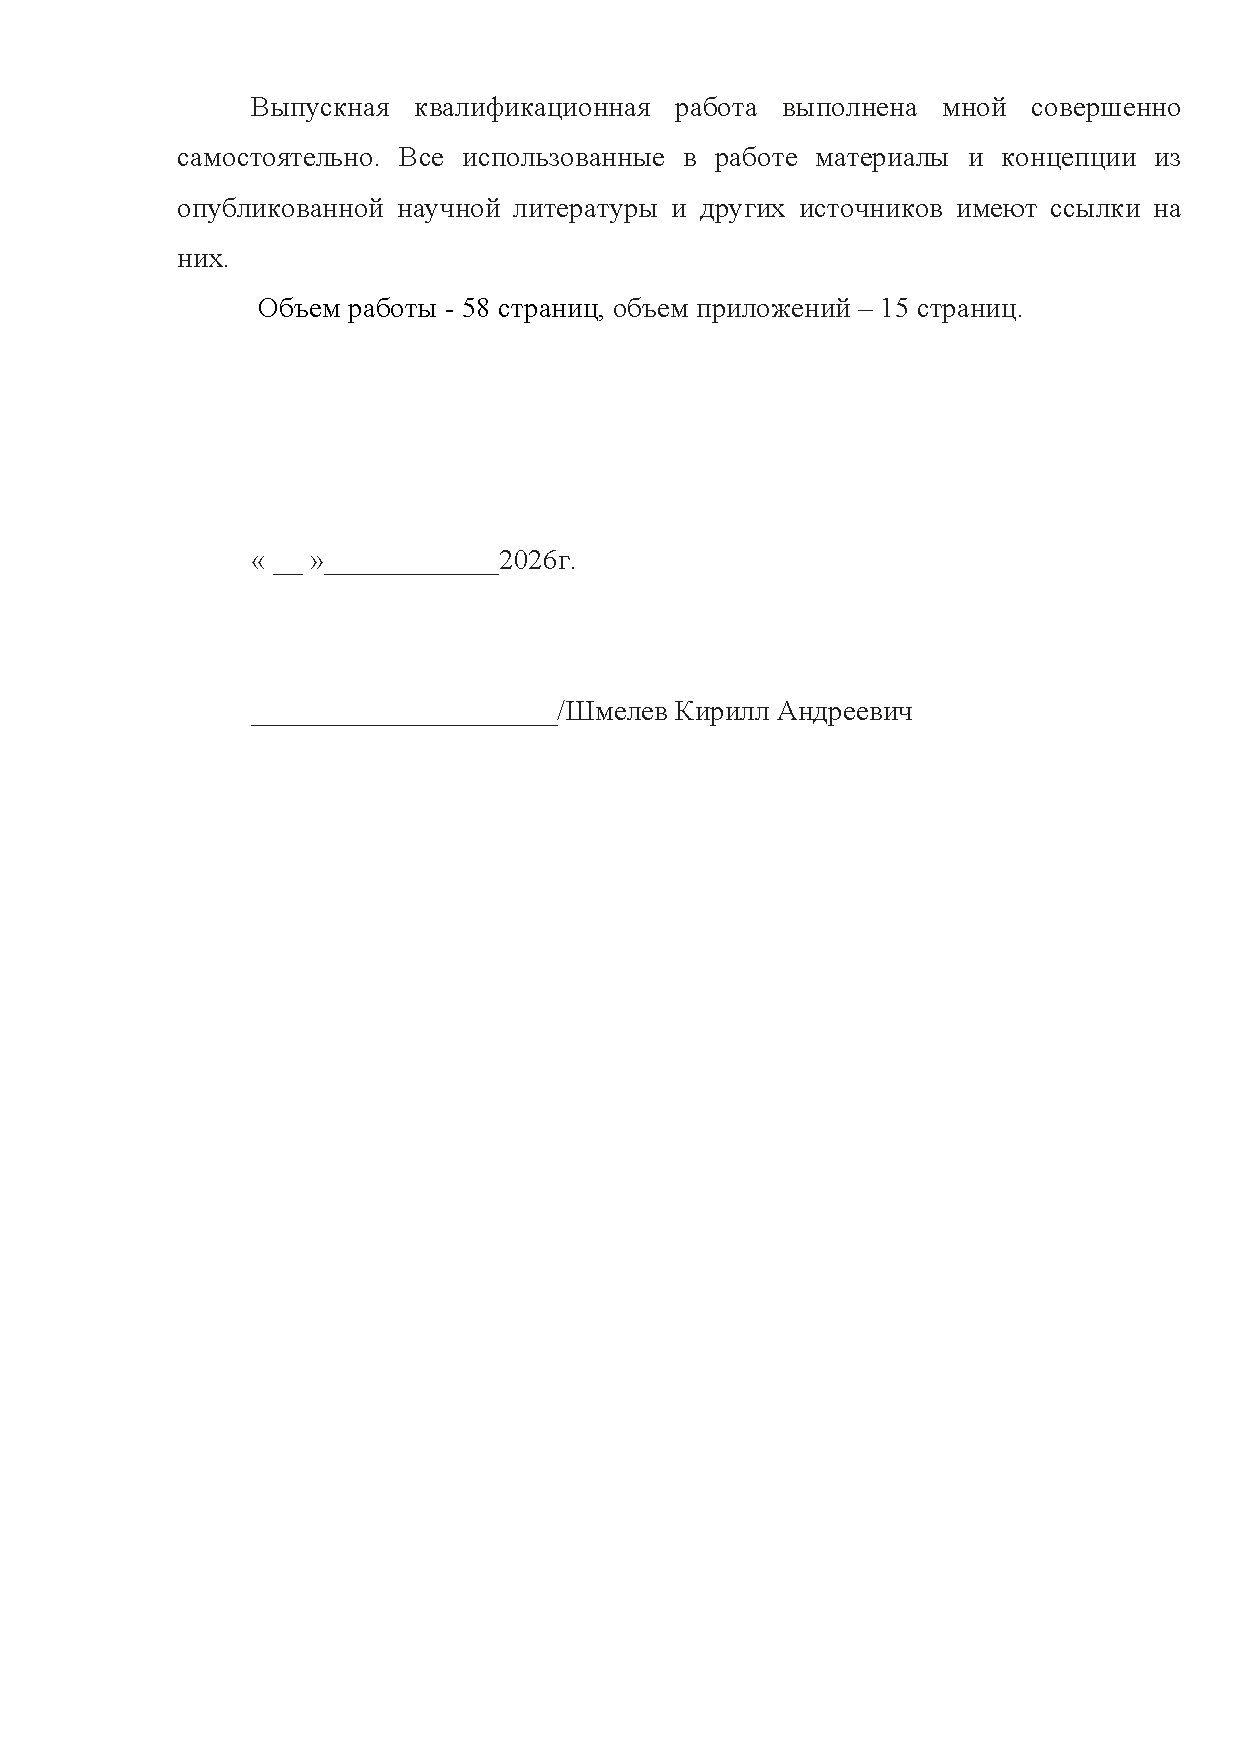
\includepdf[pages={1-1}]{extra/last.pdf}

\end{document}
